\section{Results}\label{section:Results}

A summary of all settings used for the forward and inverse calculations is presented in tables \ref{table:settings_forw} and \ref{table:settings_inv}. In the following subsections a reasoning for these parameters will be presented and results will be shown. 

\subsection{Electrical Resistivity Tomography}
For the ERT data generation 76 synthetic electrodes over a distance of 140m are used to simulate the potential differences. These values are chosen as the represent a realistic field setup as it could be done as part of a thesis work. The same reasoning is also used for the other methods. Three different electrode configurations are simulated, namely the Dipole-Dipole, Schlumberger and Wenner configuration. The noise level is defined with 2.5\% and the absolute value of 0.001mV. As the absolute noise is set very low, the data is contaminated by the relative noise magnitude. The resulting data can be visualized in terms of apparent resistivity in a pseudo section. This is shown in Figure \ref{figure:ERT_inversion_misfits} in the top row. Since no topography is considered the pseudo section already show a strong subsurface anomaly as the apparent resistivities are varying between 100$\Omega m$ and 1000$\Omega m$. We can also see that the Dipole-Dipole configuration is generating the most data points as it shows the most cells in the section. 

Using the respective inversion parameters which are stated in table \ref{table:settings_inv}. The setting for the inversion were found by trial and assumed to be good as the data misfit value $\chi$ is close to 1 for all three configurations. A data misfit of approximately 1 indicates a good data fit and is therefore desirable. The resulting true resistivity sections are presented in Figure \ref{figure:ERT_inversion_comp}. It can be seen that all three configurations do not hold significant information below a depth of 40m. They show a strong high resistivity anomaly in the centre of the section at a depth between approximately 10m and 30m that is reaching resistivities over 10000 $\Omega m$. A shallow very conductive layer is shown up to a depth of around 10m. Left and right of the strong resistive anomaly and below the conductive top layer, two layers appear. The upper one shows resistivities of around 700-1000$\Omega m$ and reaches down to approximately 20-25m. Below that a more resistive layer can be seen with up to 3000 $\Omega m$. For the Wenner configuration this region of the section appears more homogeneous with resistivies above 2000 $\Omega m$. A more detailed discussion of the final inversion results of the different ERT configurations is presented in section \ref{section:Discussion}.

\begin{figure}[H]
  \centering
    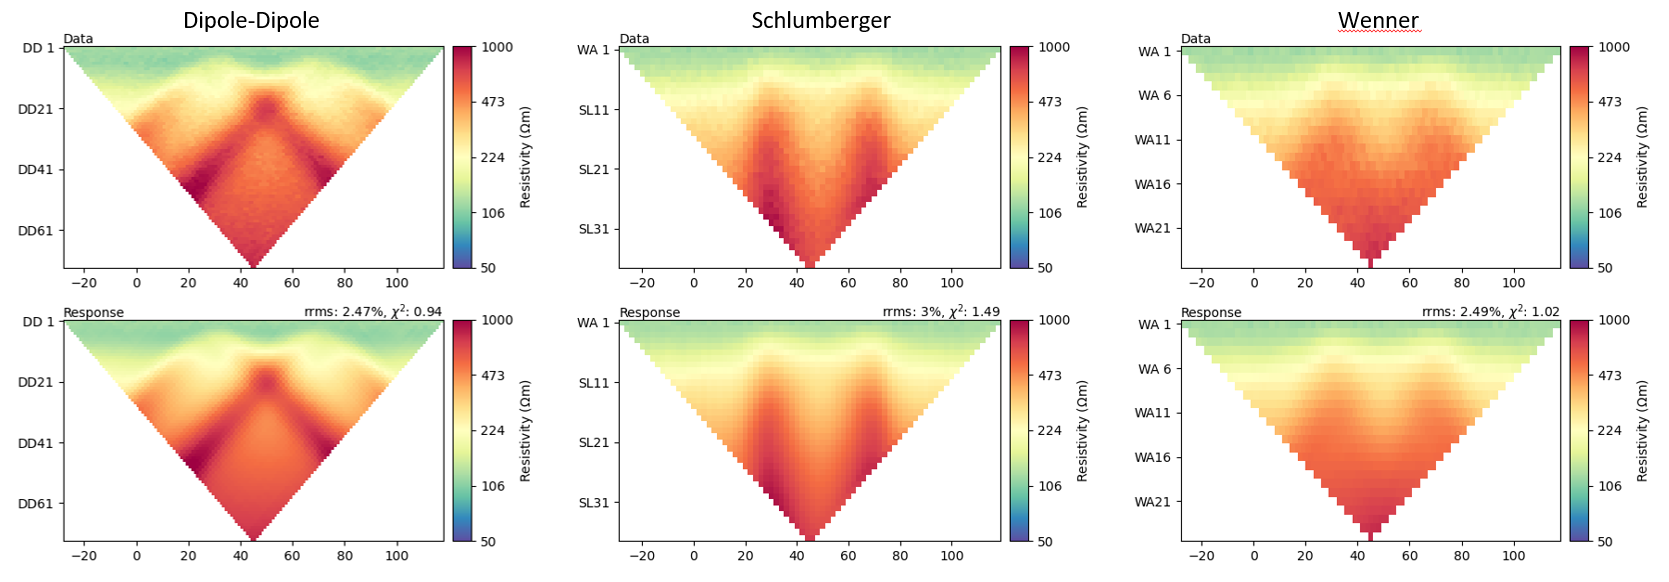
\includegraphics[width=\textwidth]{Figures/ERT_inversion_overview.png}
    \caption[ERT inversion result misfit]{Inversion result misfit of the Dipole-Dipole (left), Schlumberger (middle) and Wenner electrode configuration. At the top the synthetic data pseudo section is shown and below the pseudo section resulting from the inversion is presented. On top of the inverse model response the root mean square error (RMS) and the data misfit $\chi$ is stated.}
    \label{figure:ERT_inversion_misfits}
\end{figure}

\begin{figure}[H]
  \centering
    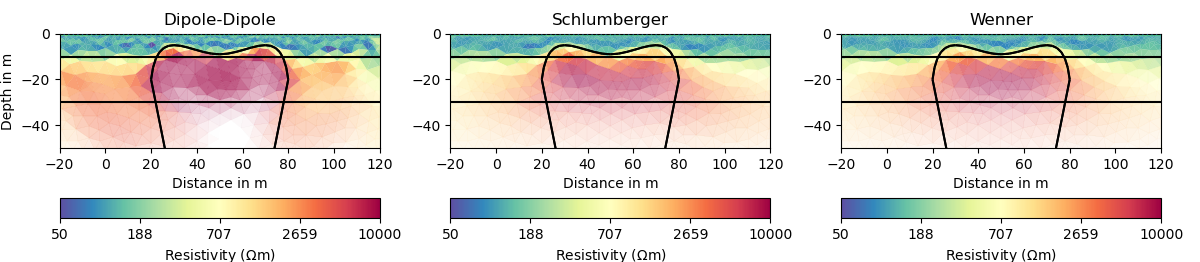
\includegraphics[width=\textwidth]{Figures/ERT_Inv_comp.png}
    \caption[Final resistivity models after inversion]{Final ERT inversion results. The results of the Dipole-Dipole (left), Schlumberger (middle) and Wenner configuration (right) are superimposed by the subsurface geometry used for synthetic data generation. The transparency of the mesh cells indicates the data coverage as opaque cells represent higher data coverage.}
    \label{figure:ERT_inversion_comp}
\end{figure}

\subsection{Traveltime Tomography}

For the traveltime tomography data generation 91 sensors with a spacing of 2m are defined between -40m and 140m. Every third sensor location is chosen to be a shot location, resulting in 31 shots. Just as the synthetic ERT data, noise is produced and added to the generated data. For the traveltime tomography the absolute noise is set to 1ms and the relative noise to 0.01\%. This means that for early arrivals, i.e. small source-receiver offsets, the absolute noise is defining the noise magnitude while for later arrivals, i.e. large offsets, the relative noise parameter is the deciding factor. The synthetic data is presented in the left part of Figure \ref{figure:TT_inversion_misfits}. In the data matrix, the zero offset measurements, i.e. measurements with an identical source and receiver location, are excluded and appear white. The simulated traveltimes are directly converted to apparent velocities using the source receiver distance.

The inversion of the traveltimes results in an estimated data matrix which is shown in the right part of Figure \ref{figure:TT_inversion_misfits}. As seen, the data misfit is very close to one and therefore a suitable inversion result can be assumed. Figure \ref{figure:TT_inversion_comp} presents the resulting velocity model on the left and the corresponding ray coverage on the right. As seen in the right plot, the data does not hold any information about the subsurface below 30m depth. In the upper 10m of the model we find a low velocity layer which holds velocities below 1000m/s. Between -20m and 20m and well as between 80m and 120m at a depth of 10m to 30m, high velocity structures appear with velocities of 3000-3500m/s. In between those high velocity anomalies two lower velocity anomalies with around 1500m/s (at a distance of 20-40m and 60-80m). Between 40m and 60m a structure with approximately 2900m/s can be observed. Further discussion of the results and a comparison with the other methods is done in section \ref{section:Discussion}.

\begin{figure}[]
  \centering
    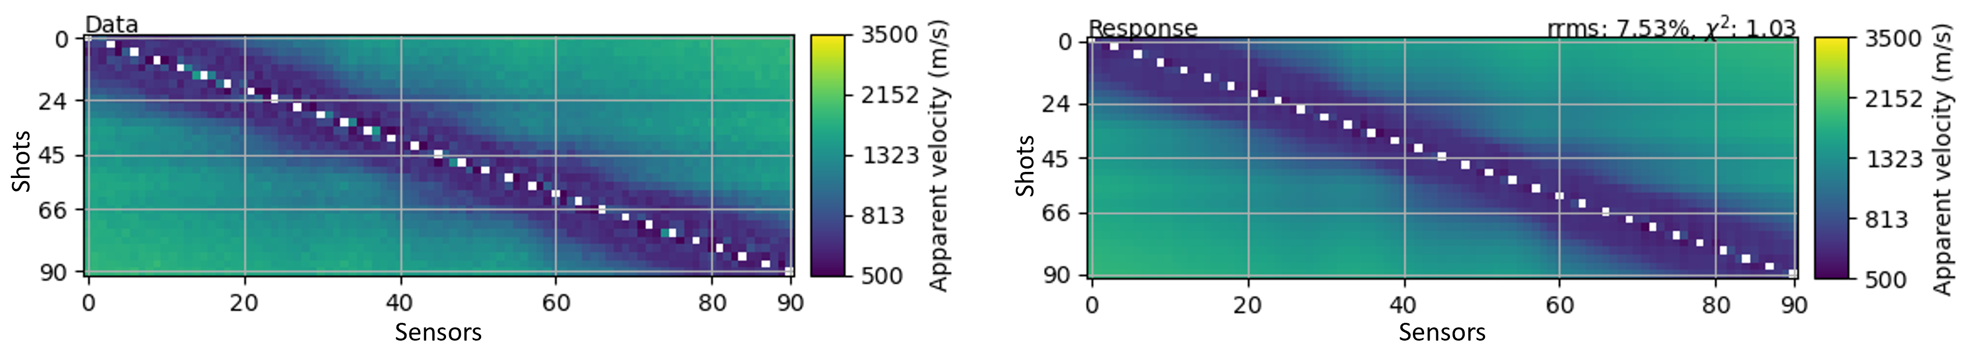
\includegraphics[width=\textwidth]{Figures/TT_RF_labels.png}
    \caption[Traveltime inversion result misfit]{Inversion result misfit of the synthetic traveltime tomography data. On the left the synthetic data is shown and on the right the estimated data resulting from the inversion is presented. On top of the inverse model response the root mean square error (RMS) and the data misfit $chi$ is stated.}
    \label{figure:TT_inversion_misfits}
\end{figure}


\begin{figure}[]
  \centering
    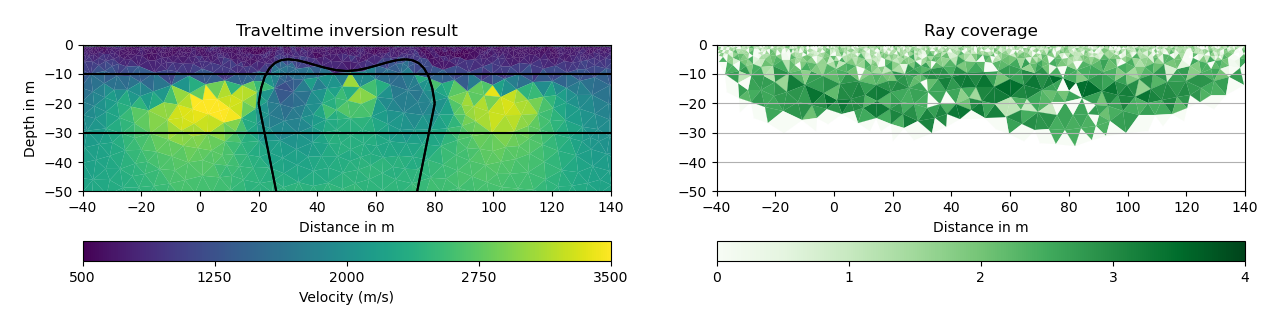
\includegraphics[width=\textwidth]{Figures/TT_comp.png}
    \caption[Final velocity model after inversion]{Final traveltime inversion results. The final velocity model (left) is superimposed by the subsurface geometry used for synthetic data generation. The ray coverage of the traveltime tomography is shown on the right.}
    \label{figure:TT_inversion_comp}
\end{figure}

\subsection{Gravimetry}
According to table \ref{table:settings_forw} the synthetic gravity data was generated using a 140m long spread of 71 stations. As no inversion is performed on these synthetic data set, no noise is generated and superimposed on the data. The synthetic gravity measurements can be seen in Figure \ref{figure:grav}. As the parameter table \ref{table:properties} states, the diatreme has a lower density than the surrounding dense sandstone and therefore also produces a negative gravity response in the synthetic data. Due to the irregular upper boundary of the diatreme structure two saddle points in the gravity anomaly can be observed at 30m and 70m. Figure \ref{figure:grav} also shows that the anomaly reaches its maximum magnitude of approximately -0.3mGal at a distance of 50m which coincides with the center axis of the diatreme structure.

\begin{figure}[]
  \centering
    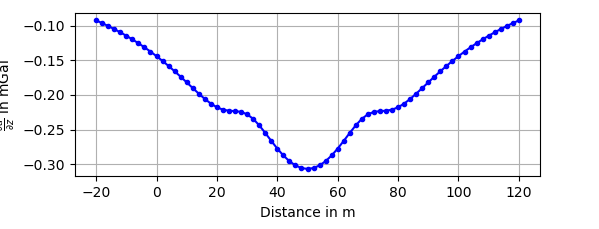
\includegraphics[width=0.6\textwidth]{Figures/GRVA_dataonly.png}
    \caption[Synthetic gravity data]{Synthetic gravity data points.}
    \label{figure:grav}
\end{figure}


